\section{Results}
\label{sec:Res}

% ----------------------------------------------------------------------- %
% ----------------------------------------------------------------------- %
\subsection{Classification Accuracies}
\label{sec:supp_tspec_res}

\subsubsection*{Effect of Support Size and Threshold}

Before calibration, the lowest user's accuracies ($UA$) for most tree species were realized using high thresholds of 80\% and 100\% for deciding the main tree species on the plot level (figure \ref{fig:supp_tspec_res}). A plausible reason for this is that raising the threshold to higher values (e.g. 80\%, 100\%) distinctively increases the probability of the reference class (based on the sample trees of the sample location) to be assigned as class 'Mixed', while the much coarser spatial resolution of the tree species map causes the $predicted$ class to remain classified as one of the five tree species. However, as the support size is  increased, so does the number of tree species raster cells to be evaluated at the sample location, thereby increasing the probability that the predicted class will be 'Mixed'. For this reason, most tree species exhibit an increase in user's accuracy under higher thresholds with higher support sizes. This scale-threshold dependency of the user's accuracy particularly affects tree species that most commonly occur in mixed forest stands in Rhineland-Palatinate (\textit{Scots pine}, $oak$ and $beech$), whereas the user's accuracies for tree species that are mostly prominent in pure forest stands ($spruce$, \textit{Douglas fir}) logically turned out to be much more robust to changes in the thresholds and support sizes.\par
Among the uncalibrated tree species predictions, $beech$ and $spruce$ produced the best predictions achieving UAs of up to 70\% and 80\%.  Although the predictions for \textit{Douglas fir} and \textit{Scots pine} generally performed less well than $beech$ and $spruce$, similar UAs can be produced by adjusting the threshold and support choices. UAs for $oak$ never performed better than 50\%. A detailed table of the user's and overall accuracies is provided in Online Resource 3.

\begin{figure}[H]
\centering
\subcaptionbox{\label{fig:supp_tspec_res}}{%
  
\includegraphics[width=0.4\textwidth]{cos_tspec_mixed_cal_nocal.png}%
  }\par\medskip
\subcaptionbox{\label{fig:supp_tspec_oaa_res}}{%
  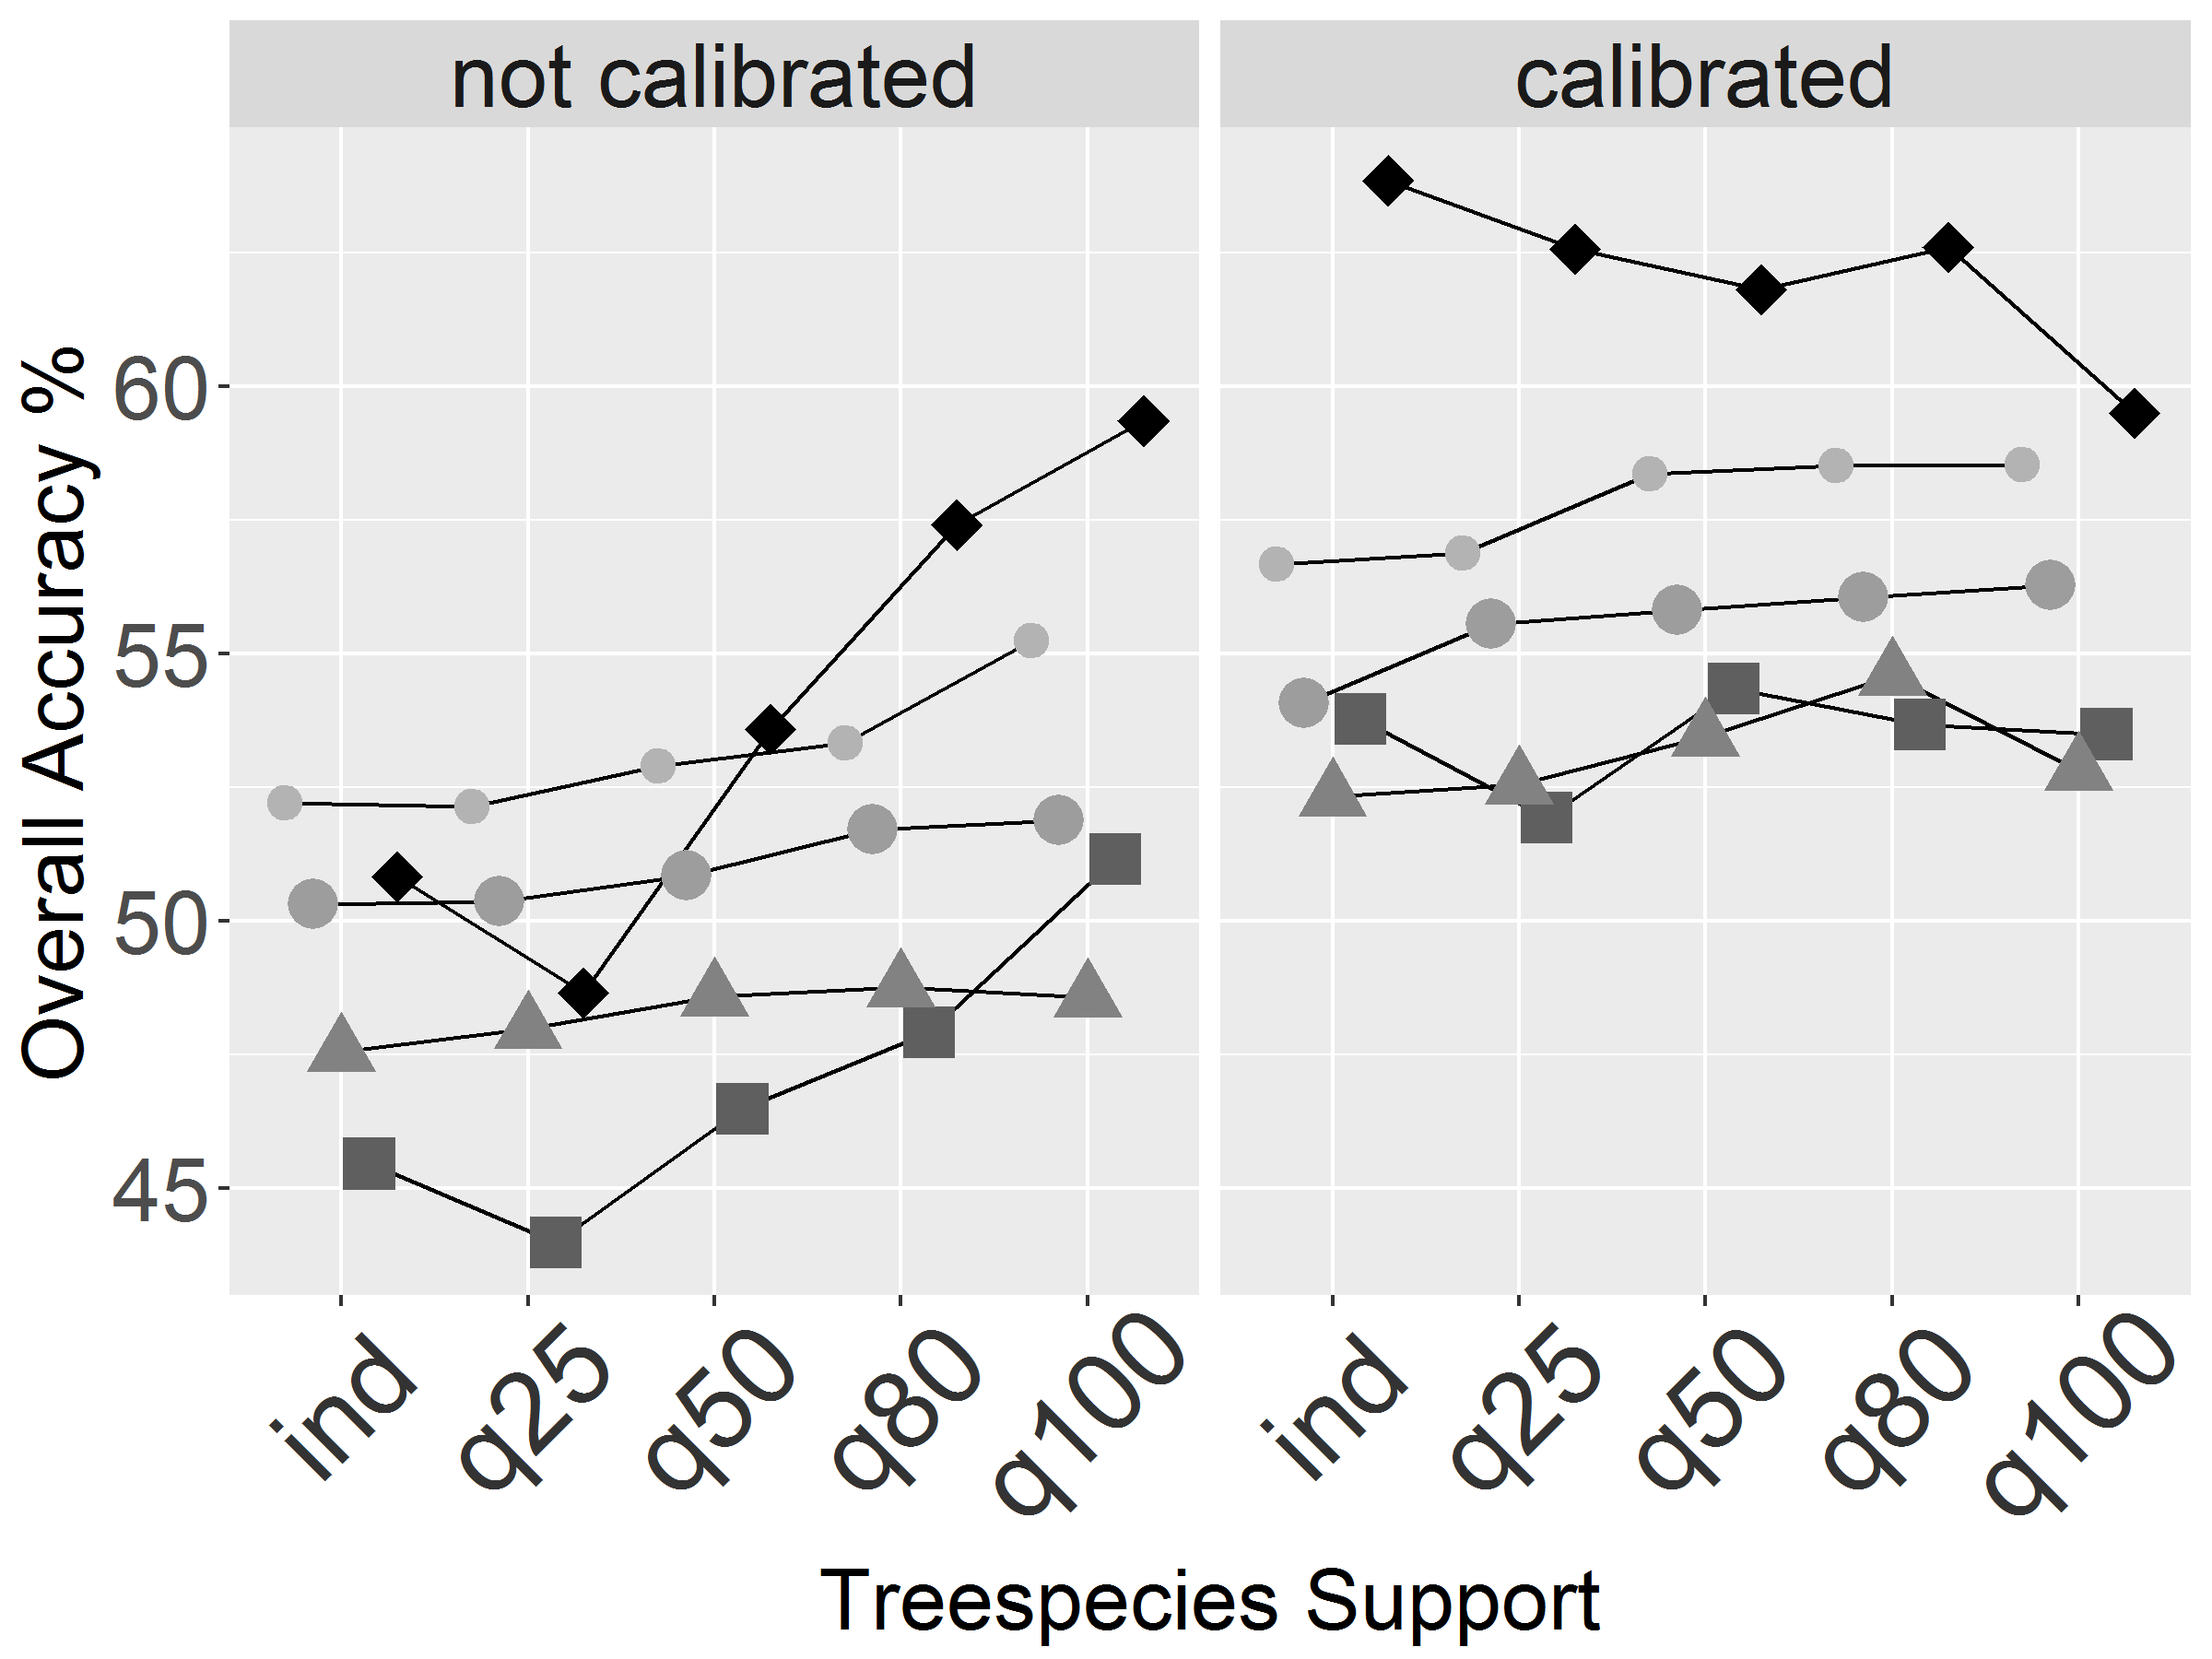
\includegraphics[width=0.4\textwidth]{cos_tspec_oaa_mixed.png}%
  }\par\medskip
\caption{Classification accuracy for the main tree species of a sample location \textit{before} and \textit{after} calibration: \textit{a)} user's accuracies. \textit{b)} overall accuracies. $n$: number of validation data per class}
\label{fig:cos_oaa_ua}
\end{figure}


\subsubsection*{Effect of Calibration}
Calibration substantially diminished the effect of the scale-threshold dependency for the five tree species and also increased the UAs for \textit{Scots pine} and $oak$. Whereas the UA level of $spruce$ remained unchanged, the UAs for $beech$ were found to be slightly lower after calibration. The overall accuracy under each support choice was always considerably increased by calibrating the tree species prediction (figure \ref{fig:supp_tspec_oaa_res}). With respect to the calculated random forest models, the initial tree species prediction ($treespecies$) and the information about the growing region ($wgb$) turned out to be the most valuable information, followed by the estimated proportion of coniferous trees ($prop.conif$) and the mean canopy height ($meanheight$).


% ----------------------------------------------------------------------- %
% ----------------------------------------------------------------------- %
\subsection{Regression Model Accuracies}
\label{sec:supp_chm_tspec_res}


\subsubsection*{Effect of Support Size and Threshold}

Figure \ref{fig:supp_perf_res} shows the accuracies of the regression model (equation \ref{eq:chmtspec_fullmod_term}) achieved under all possible combinations of support sizes for the auxiliary data. The stepwise selection procedure always included all considered single and interaction terms. In terms of \adjrsq{} and \rmsecv{}, the analysis revealed that the choice of the CHM support size controls the overall level of the model's accuracy. The information about the main plot tree species can then be used to further improve the model fit under suitable $treespecies$ support and threshold settings. When using the uncalibrated $treespecies$ variable, an increase of the $treespecies$ support size causes an increase in the model performance if low thresholds are used, whereas high thresholds (80\%, 100\%) cause a decrease in the model performance. This threshold-dependency could be removed by calibrating the $treespecies$ variable. The highest \adjrsq{} and the lowest \rmsecv{} were realized using the $q50$ support for the CHM variables in combination with the $q100$ support and a threshold of 100\% for the calibrated $treespecies$ variable (\adjrsq{}=0.48 and \rmsecv{}=137 \mha{}). However, various support and threshold combinations for the CHM and $treespecies$ variables can be used to yield almost identical \rmsecv{} and \adjrsq{} values. A detailed table of the model accuracies is given in Online Resource 4.

\begin{figure*}
\centering
\resizebox{0.8\hsize}{!}{\includegraphics*{cos_cal_nocal_bw.png}}
\caption{10-fold \rmsecv{} and \adjrsq{} realized under various support choices for the CHM and $tree species$ explanatory variables}
\label{fig:supp_perf_res}
\end{figure*}



\subsubsection*{Effect of Misclassifications}

We can assess magnitude of the misclassification effect by comparing the \adjrsq{}'s of models that use the predicted tree species (calibrated and uncalibrated) as an explanatory variable to models that use the error-free tree species variables acquired from the terrestrial survey. Note that only the model with the predicted tree species variables can be applied to additional sample locations where no terrestrial survey has been carried out. Figure \ref{fig:supp_r2_calnocal} provides a comparison of the \adjrsq{} achieved under the use of the error-free tree species predictor variable against the \adjrsq{} realized under the use of the tree species variable containing missclassifications. This analysis was carried out for all models that were analysed in section \ref{sec:supp_chm_tspec_res}, i.e. for all possible support and threshold combinations for the CHM and $treespecies$ predictor variables.\\
As expected, the highest \adjrsq{} for every evaluated model was always achieved using the error-free tree species variable, whereas the missclassifications in the tree species variable led to a systematic decrease of the model accuracy. This is in agreement with the potential effects of erroneous explanatory variables discussed in \citet{carroll2006} and \citet{gustafson2003}, i.e. an increase of variability (noise) in the data that can increase the amount of unexplainable variance and thereby reduce the model accuracy.\\
The calibration of the initially predicted main plot tree species using the random forest classification algorithm (section \ref{sec:tspecclass}) turned out to not only improve the classification accuracies (section \ref{sec:supp_tspec_res}), but also to considerably decrease the effect of the missclassifications on the regression model predictions and accuracy. Figure \ref{fig:supp_r2_calnocal} ($right$) shows that the \adjrsq{} under the actual and the calibrated predicted tree species variable are in general much closer to, and in many cases even on the identity line. Whereas the misclassifications in the uncalibrated $treespecies$ variable led to a residual inflation of 1\% - 5\%, it was only between 0\% and 1\% after calibration. Further analysis revealed that when using the calibrated $treespecies$ variables, the regression coefficients were almost identical to the ones received using the actual main plot tree species.

\begin{figure*}
\centering
\resizebox{0.65\hsize}{!}{\includegraphics*{cos_r2_cal_vs_nocal.png}}
\caption{Effect on the \adjrsq{} when substituting the actual main tree species with the predicted  main tree species of a sample plot. The differentiation into two distinct point clouds results from the poor model performance under support size $q100$ for the CHM variables (i.e. the $lower$ point cloud). The \textit{dotted} line tracks the the model with the highest \adjrsq{} under the use of the error-free \textit{treespecies} variable}
\label{fig:supp_r2_calnocal}
\end{figure*}


% ----------------------------------------------------------------------- %
% ----------------------------------------------------------------------- %
\subsection{Final Regression Model}
\label{sec:regmod_final}

In order to address research questions 1 and 2 (i.e. the gain in model accuracy by tree species information and effect of heterogeneity in the LiDAR data), we investigated the model properties in more detail. For this purpose, we decided to use the support settings of $q50$ for both auxiliary data with a threshold of 100\% for the tree species variable as the regression model of choice. The reason for this choice was that \textit{a)} the model provided almost the highest \adjrsq{} among all validated models while reducing the data handling complexity for upcoming applications (i.e. identical support sizes for all remote sensing data) and \textit{b)} the calibration neutralized the effects of misclassifications on the model predictions. The interaction term between $meanheight^2$ and $treespecies$ (i.e. considering separate curvatures for each tree species) turned out not to have any influence on the model accuracy and was thus dropped, resulting in an \adjrsq{} of 0.49 and \rmsecv{} of 132.12 m$^2$/ha.

\subsubsection*{Interpretation of Final Regression Model}
\label{sec:prop_regmod_final}
Figure \ref{fig:predlines_tspec} provides a visualisation of the tree species prediction functions separated by the LiDAR acquisition years. Sample plots classified as $oak$ and \textit{Scots pine} revealed to have an almost identical relationship (nearly identical slopes) for the mean canopy height - timber volume relationship. They only differ by a marginally higher intercept for \textit{Scots pine} plots, meaning that given the same mean canopy height a sample plot dominated by \textit{Scots pine} yields a marginally higher timber volume on the plot level than a plot dominated by $oak$. $Beech$-dominated sample plots tend to achieve a higher timber volume than $oak$ and \textit{Scots pine} for canopy heights below 20 meters, but realize the lowest timber volumes for canopy heights above 20 metres. Sample plots dominated by any of the remaining coniferous tree species (\textit{Douglas fir}, $spruce$) revealed to have higher slopes than broadleaf classified plots. This indicates that given the same mean canopy height, sample plots dominated by \textit{Douglas fir} and $spruce$ yield higher timber volume values than broadleaf- or \textit{Scots pine} dominated sample plots, and this difference becomes more pronounced with increasing mean canopy heights. Within the group of coniferous-dominated sample plots, $spruce$ turned out to have the highest slope, thereby yielding the highest timber volume values for mean canopy heights above 15 meters. An undesired characteristic of the model is that the predicted timber volume can in some cases ($<$ 1\%) take negative values for low canopy heights (e.g. for $spruce$-dominated plots with \textit{meanheight} below 5 meters and $stddev$ of 4 meters). However, we chose not to use a log-transformation of the response variable. Doing so would have prevented the subsequent calculation of the g-weight variance of the model assisted estimators \citep{mandallaz2013a, mandallaz2013b}, which is only possible for response variables on the original scale.

\begin{figure*}[h]
\centering
\resizebox{0.8\hsize}{!}{\includegraphics*{predlines_tspecaux_cal.png}}
\caption{Visualization of the timber volume prediction function (\textit{final regression model}) on sample plot level for each main plot tree species and LiDAR acquisition year. For visualization purposes, the predictor variable $stddev$ was set to its average value within the respective \textit{treespecies} and \textit{lidaryear} group}. The terrestrially observed timber volume values are plotted in the background.
\label{fig:predlines_tspec}
\end{figure*}


\subsubsection*{Effect of Time-Lags and Heterogeneity in LiDAR Data}

Incorporating the LiDAR acquisition year as a categorical variable ($lidaryear$) in the regression model substantially accounted for the variability in the data introduced by \textit{a)} the time-lags between LiDAR acquisition and terrestrial survey, and \textit{b)} variation in LiDAR data quality which are due to sensor- and post processing techniques (table \ref{tab:modacc_modterms}). Whereas the \adjrsq{} for the regression model without considering the LiDAR acquisition year as additional predictor variable was 0.35 (0.40 including the tree species variable), the stratification by the LiDAR acquisition year led to \adjrsq{} of 0.44 (0.48), thereby increasing the proportion of explained variance by up to 8\%.

\begin{figure}[H]
\centering
\resizebox{1\hsize}{!}{\includegraphics*{r2adj_in_lyears.png}}
\caption{$R^2$ of the final regression model achieved $within$ the LiDAR acquisition year strata. 
         \textit{Grey points}: $R^2$ of submodel 1 (no stratification according to LiDAR acquisition year or tree species). 
         $Crosses$: $R^2$ of submodel 2 ($without$ tree species stratification). 
         \textit{Filled triangles}: $R^2$ of final model using the $uncalibrated$ tree species variable.
         \textit{Empty triangles}: $R^2$ of final model using the $calibrated$ tree species variable.
         $Diamonds$: $R^2$ achieved using the error-free tree species variable (derived from sample trees).
         \textit{Dotted line}: Overall \adjrsq{} of submodel 2.
         \textit{Solid line}: Overall \adjrsq{} of final model using the $calibrated$ tree species variable.
         \textit{Two-dashed line}: Overall \adjrsq{} of final model using the \textit{error-free} tree species variable}
\label{fig:r2adj_in_lyears}
\end{figure}

% latex table generated in R 3.4.2 by xtable 1.8-2 package
% Sun Jan 07 17:26:28 2018
\begin{table}[ht]
	\centering
	\caption{$R^2$, RMSE and RMSE\% of final regression model within ALS acquisition year strata (\textit{ALSyear}). $Area_{ALSyear}$: Area covered by ALS acquisition given in km$^2$. \textit{n}: number of validation data.}
	\label{tab:adj_r2_within}
	\begin{tabular}{lllrrr}
		\hline
		\textit{ALSyear} & $Area_{ALSyear}$ & $R^2$ & RMSE & RMSE\% & n \\ 
		\hline
 2012 & 2807   & 0.61 & 135.84 & 44.87 & 408 \\ 
 2011 & 4361  & 0.57 & 146.21 & 48.29 & 883 \\ 
 2010 & 4182 & 0.51 & 120.90 & 39.93 & 1171 \\ 
 2009 & 2100 & 0.42 & 133.42 & 44.07 & 559 \\ 
 2008 & 2968 & 0.48 & 130.38 & 43.06 & 701 \\ 
 2008\_1 & 2116 & 0.33 & 175.43 & 57.94 & 394 \\ 
 2007 & 3498 & 0.46 & 136.47 & 45.08 & 418 \\ 
 2003 & 602 & 0.27 & 154.48 & 51.02 & 529 \\ 
 2002 & 775 & 0.44 & 141.55 & 46.75 & 314 \\ 
		\hline
\hline
\end{tabular}
\end{table}
%\end{longtable}
%\endgroup

%% old version
%\begin{table}[ht]
%	\centering
%	\caption{$R^2$, RMSE and Residual Square Sum (SSE) of final regression model within LiDAR acquisition year strata (\textit{lidaryear}). \textit{n}: number of validation data}
%	\label{tab:adj_r2_within}
%	\begin{tabular}{llrrr}
%		\hline
%		LiDAR acquisition year & $R^2$ & rmse & SSE & n \\ 
%		\hline
%		2012   & 0.55 & 139.54 & 7535278 & 387 \\ 
%		2011   & 0.55 & 145.21 & 17880553 & 848 \\ 
%		2010   & 0.48 & 122.16 & 16907662 & 1133 \\ 
%		2009   & 0.43 & 127.17 & 8652419 & 535 \\ 
%		2008\_1 & 0.34 & 170.49 & 11161424 & 384 \\ 
%		2008   & 0.50 & 124.39 & 10475374 & 677 \\ 
%		2007   & 0.49 & 129.72 & 6950192 & 413 \\ 
%		2003   & 0.32 & 146.37 & 11139814 & 520 \\ 
%		2002   & 0.43 & 139.79 & 6038601 & 309 \\ 
%		\hline
%		\hline
%	\end{tabular}
%\end{table}
%%\end{longtable}
%%\endgroup


We further analysed the model residuals within each LiDAR acquisition year (within-group variation) for the final model and nested submodels. It turned out that the $R^2$ vary distinctly between the LiDAR acquisition year strata (figure \ref{fig:r2adj_in_lyears}). More precisely, the within-group $R^2$ can be higher and lower than the overall $R^2$ of the respective model. Figure \ref{fig:r2adj_in_lyears} shows that a stratification according to the LiDAR acquisition years (submodel 2) can already increase the $R^2$ in most acquisition year strata, compared to the basic model using only the LiDAR height metrics as predictor variables (submodel 1). In some LiDAR acquisition year strata (i.e. 2007, 2008), this increase in $R^2$ even reached 7\% - 11\%. The accuracies for the final model are also given in table \ref{tab:adj_r2_within}.


\subsubsection*{Added Value of Tree Species Map Information}

%% Second submission version:
Introducing the predicted main tree species of a sample plot as an additional categorical variable to submodel 2 yielded a further 4\% increase in the \adjrsq{} (table \ref{tab:modacc_modterms}). This improvement was even more pronounced in LiDAR acquisition years close or identical to the year of the terrestrial inventory (up to 7\% increase in $R^2$, figure \ref{fig:r2adj_in_lyears}. The analysis illustrated once more that misclassifications in the tree species variable generally reduce model accuracy compared to using error-free tree species information. The residual inflations caused by the misclassifications in the uncalibrated $treespecies$ variable within the $lidaryear$ strata were up to 5\%. However, the calibration was able to substantially decrease or even remove the effects of misclassifications on the model accuracy in all LiDAR acquisition year strata.

%% OLD (first submission version):
%Using the predicted main tree species of a sample plot as an additional categorical variable yielded a further increase of the model accuracy of 5\% in the $R^2$ (table \ref{tab:modacc_modterms}). This improvement was particularly pronounced in LiDAR acquisition years that are close or identical to the year of the terrestrial inventory ($R^2$ of 0.55 in 2011 and 2012, figure \ref{fig:r2adj_in_lyears}). The analysis illustrated once more that misclassifications in the tree species variable generally reduce model accuracy compared to using error-free tree species information. The residual inflations caused by the misclassifications in the uncalibrated $treespecies$ variable within the $lidaryear$ strata were up to 5\%. However, the calibration was able to substantially decrease or even remove the effects of misclassifications on the model accuracy in all LiDAR acquisition year strata.

%format: onecolumn
% \begingroup\fontsize{10pt}{11pt}\selectfont
\begin{table*}
\centering
\caption{Accuracy metrics for submodels of final OLS regression model} 
\label{tab:modacc_modterms}
\begin{tabular}{llrrr}
  \hline
model terms & model & parameters & $R^2_{adj}$ & \rmsecv{} \\ 
  \hline
meanheight + stddev + meanheight$^2$ + \\ treespecies + lidaryear + meanheight:treespecies + \\ meanheight:lidaryear + meanheight:stddev + \\ stddev:lidaryear & final model &  39 & 0.48 & 137.49 \\ \\
  meanheight + stddev + meanheight$^2$ + \\ meanheight:stddev & submodel 1 &   5 & 0.35 & 153.02 \\ \\
  meanheight + stddev + meanheight$^2$ + \\ lidaryear + meanheight:lidaryear + \\ meanheight:stddev + stddev:lidaryear & submodel 2 &  29 & 0.44 & 142.82 \\ \\
  meanheight + stddev + meanheight$^2$ + \\ treespecies + meanheight:treespecies + \\ meanheight:stddev & submodel 3 &  15 & 0.40 & 142.82 \\ 
   \hline
\hline
\end{tabular}
\end{table*}
%\endgroup

























